\chapter{Proof of Concept Prototype V1}
\label{poc1:chapter}
In diesem Kapitel wird folgende Frage beantwortet: \textit{''Ist eine praxistaugliche Software, die die Problemstellung des Auftrags erfüllt, möglich?''}.\\

Dieser Prototyp V1 setzt auf die Architektur der Echtzeit Erkennung.

%ANF

\begin{table}[H]
	\section{Anforderungen}
    \centering
	\begin{tabularx}{\textwidth}{| l | X |}
        \hline
        \textbf{ANF-Nummer} & \textbf{Beschreibung} \\ \hline
        \textbf{P1-ANF01} & Der Proxy durchsucht die Pakete nach Malware Eigenschaften. \\ \hline       
        \textbf{P1-ANF02} & Der Proxy leitet Pakete mit Malware Eigenschaften auf einen Fake \gls{cc} Server um. \\ \hline  
        \textbf{P1-ANF03} & Der Proxy ist ein SSL Splitting Proxy, um HTTPS Pakete zu entschlüsseln. \\ \hline
        \textbf{P1-ANF04} & Der Client sendet Pakete mit Malware Eigenschaften. \\ \hline       
        \textbf{P1-ANF05} & Der Client unterstützt HTTPS.  \\ \hline        
        \textbf{P1-ANF06} & Der Fake \gls{cc} Server unterstützt HTTPS.  \\ \hline  
        \textbf{P1-ANF07} & Der Redirect wird gesetzt, bevor das Paket den Proxy verlässt, so dass das Paket sofort umgeleitet wird. \\ \hline     
    \end{tabularx}
    \caption{Prototyp V1: Anforderungen}
\end{table}
%ANF


%NFRs
\begin{table}[H]
	\section{Nicht Funktionale Anforderungen}
    \centering
	\begin{tabularx}{\textwidth}{| l | X |}
        \hline
        \textbf{NFR-Nummer} & \textbf{Beschreibung} \\ \hline
        \textbf{P1-NFR01} & Der Benutzer darf keine Verschlechterung der Performance durch das System beim Benutzen des Netzwerks bemerken. \\ \hline        
    \end{tabularx}
    \caption{Prototyp V1: Nicht Funktionale Anforderungen}
\end{table}
%NFRs
\newpage
%Use Cases
\section{Use Cases}
Die Use Cases sind nur für den Prototyp V1 gültig und sind deshalb mit dem Pattern "P1" gekennzeichnet.

\begin{table}[H]
	\subsection{P1-UC01: Pattern erkennen}
    \centering
    \begin{tabularx}{\textwidth}{| l | p{0.6\textwidth} |}
        \hline
        \textbf{Use-Case-Name}     & \textbf{Pattern erkennen}    \\ \hline
        \textbf{Umfang}  & Fiddlercore Proxy     \\ \hline
        \textbf{Ebene} & Unterfunktionsebene   \\ \hline
        \textbf{Primärakteur} & Fiddlercore Proxy \\ \hline
        \textbf{Vorbedingungen} & Fiddlercore Proxy als zentraler Proxy konfiguriert \\ \hline
        \textbf{Nachbedingungen} & Umleitung gesetzt (P1-UC02) \\ \hline
        \textbf{Standardablauf} & \begin{enumerate}
        	\item Netzwerkpaket trifft beim Fiddlercore Proxy ein.
        	\item Paket wird auf Pattern geprüft.
        	\item Command \& Control Pattern erkannt.
        	\item IP Adresse umleiten.
        \end{enumerate} \\ \hline
        \textbf{Offene Fragen} & \begin{itemize}
        	\item Wie kann der verschlüsselte Payload von der Malware erkannt und entschlüsselt werden?
        \end{itemize} \\ \hline
    \end{tabularx}
    \caption{Prototyp V1: P1-UC01 Pattern erkennen}
\end{table}


\begin{table}[H]
	\subsection{P1-UC02: Umleitung setzen}
    \centering
    \begin{tabularx}{\textwidth}{| l | p{0.6\textwidth} |}
        \hline
        \textbf{Use-Case-Name}     & \textbf{Umleitung setzen}    \\ \hline
        \textbf{Umfang}  & Fiddlercore Proxy     \\ \hline
        \textbf{Ebene} & Unterfunktionsebene   \\ \hline
        \textbf{Primärakteur} & Fiddlercore Proxy \\ \hline
        \textbf{Vorbedingungen} & Fiddlercore Proxy als zentraler Proxy konfiguriert \\ \hline
        \textbf{Nachbedingungen} & IP Adresse für Umleitung gespeichert \\ \hline
        \textbf{Standardablauf} & \begin{enumerate}
        	\item IP Adressen speichern.
        	\item Bei Eintreffen eines Pakets mit der gespeicherten IP wird das Paket auf den Fake Command \& Control Server umgeleitet.
        \end{enumerate} \\ \hline
    \end{tabularx}
    \caption{Prototyp V1: P1-UC02 Umleitung setzen}
\end{table}
%Use Cases

%Design
\section{Design}
Der Prototyp V1 wurde mit dem Framework Fiddler Core\cite{fiddler:doku} \cite{ fiddler:book} \cite{fiddler:apidoku} implementiert, der eine grosse Bandbreite an Funktionen hat.
Bei dem Framework handelt es sich um eine .NET Bibliothek, daher wurde der Fake C\&C und der Client ebenfalls in C\#\cite{msdn} geschrieben.

\begin{figure}[H]
	\subsection{Deployment Diagramm}
	\centering
	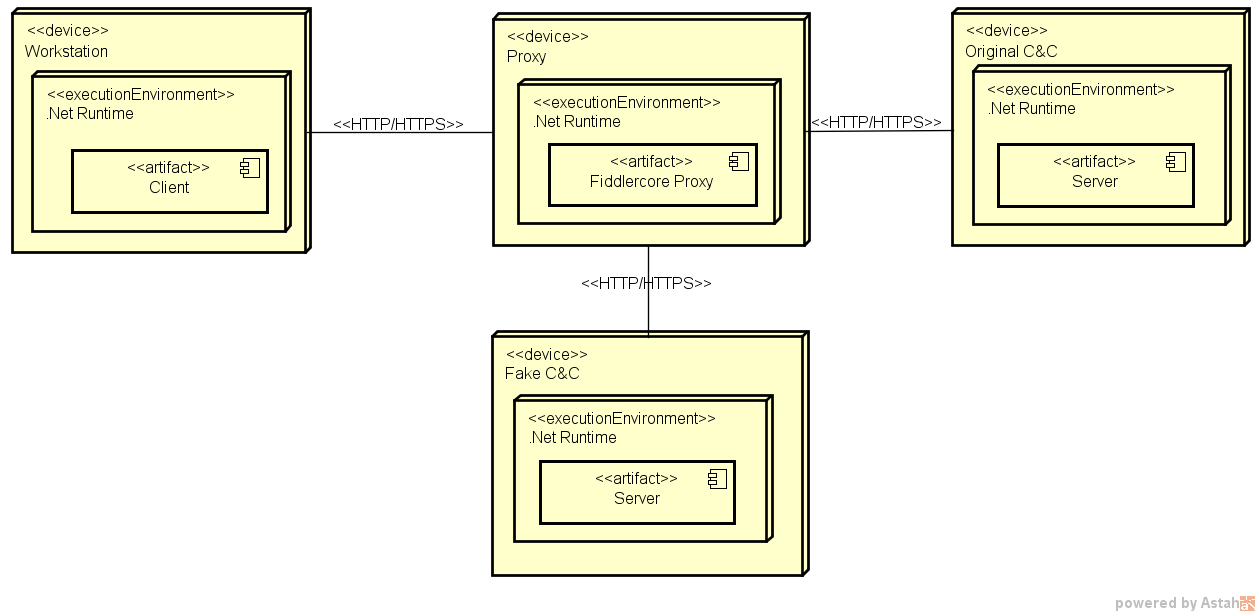
\includegraphics[width=0.85\textwidth]{img/PrototypeV1.png}
	\caption{Prototyp V1: Deployment Diagramm}
	\label{fig:deployment-Diagramm-prototyp-v1}
\end{figure}


\subsection{Proxy}
Der Proxy überprüft das Paket, das vom Client gesendet wird, auf einen vorhandenen Trojan-Header.

\begin{listing}[H]
\begin{csharpcode}
//Redirect according to Trojan-Header
if (oS.oRequest.headers.Exists("Trojan")) oS.host = "127.0.0.1:9443";
\end{csharpcode}
\caption{Prototyp V1: Beispielcode für Umleitung in Fiddler}
\label{lst:fiddler-core}
\end{listing}

Bei der Umleitung muss beachtet werden, ob es sich um eine HTTP oder HTTPS Verbindung handelt, damit sie auf den richtigen Port umgeleitet werden kann.

\subsection{Fake C\&C}
\label{protv1:fakecc}
Der Fake C\&C ist ein einfacher HTTP/HTTPS Server, der auf die Requests des Clients mit einem einfachen 200 OK Response antwortet.

\subsection{Client}
\label{protv1:client}
Der Client sendet zufällige HTTP und HTTPS Requests an den Proxy und fügt einzelnen Requests einen Trojan-Header hinzu, nach welchem beim Proxy gefiltert wird.

\begin{figure}[htbp!]
	\subsection{System Sequenz Diagramm eines Redirects}
	\centering
	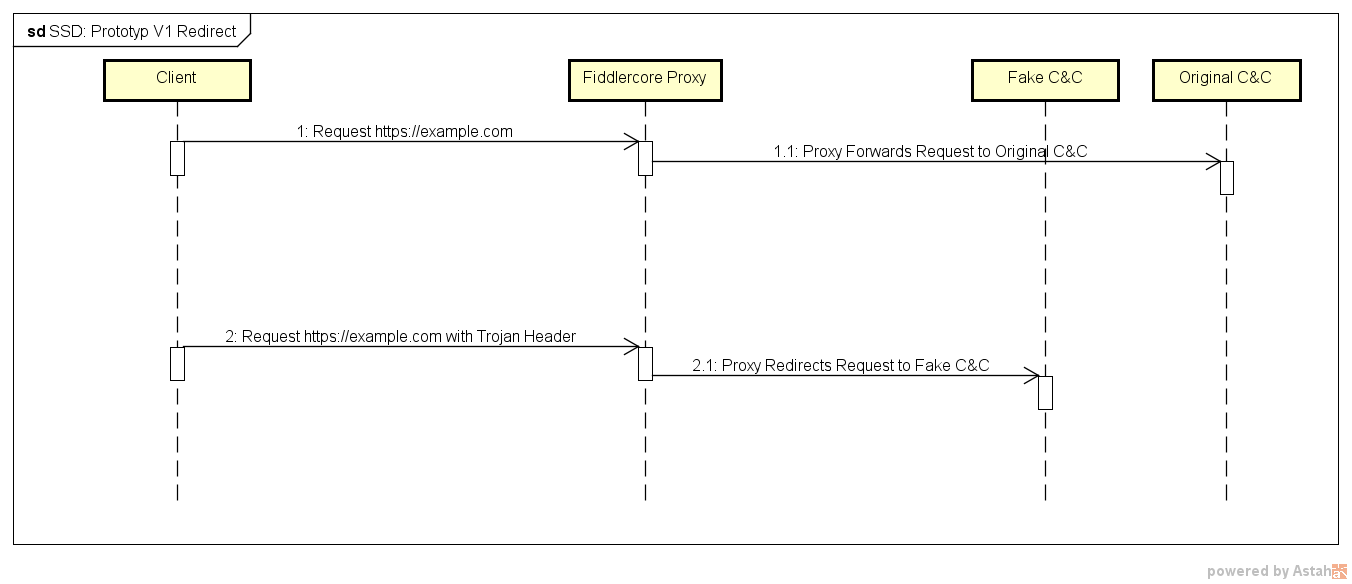
\includegraphics[width=\textwidth]{img/ssd.png}
	\caption{Prototyp V1: System Sequenz Diagramm Redirect}
	\label{fig:SSD: Prototyp V1 Redirect}
\end{figure}


%Design



\newpage
%Schlussfolgerung
\section{Schlussfolgerung}
Der Proxy besitzt viel Logik, was zu Problemen bei Performance und Wiederverwendbarkeit führt. Wenn das System in einer Firma integriert werden soll, die keine Änderungen an ihrem Netzwerk vornehmen will, dann ist eine Integration nicht möglich.
Hier sollte wenn möglich alles aufgetrennt werden, damit nicht eine einzige Stelle so viele Verantwortlichkeiten besitzt (Separation of Concern).

Im Abschnitt \ref{pocvalid:v1} wurde die Validation des Prototyp V1 durchgeführt, auf welcher die nachfolgende Entscheidung aufbaut.

\subsection{Entscheidung}
Aus genannten Gründen wird nach einer bessere aufgetrennten Lösung gesucht, und da der Host zu Beginn (falls HTTPS) bekannt sein muss, wird es nicht möglich sein, alle Requests in Real Time umleiten zu können.
Das hat uns veranlasst, eine Zeitversetzte Erkennung zu entwickeln und dabei die Zuständigkeiten aufzutrennen, um bessere Performance und Wiederverwendbarkeit zu erhalten.







